\documentclass[12pt]{article}

\usepackage{a4wide}
\usepackage{graphics}
\usepackage{amsfonts}
\usepackage{amsmath, amssymb, amsthm}
\usepackage{epsfig}
\DeclareGraphicsRule{.tif}{png}{.png}{`convert #1 `dirname #1`/`basename #1 .tif`.png}
\usepackage{caption}
\usepackage{subcaption}
\usepackage[ngerman]{babel}
\usepackage{hyperref}

\title{- KV4 - \\ Zählen einzelner Photonen mit einem Silicon Photomultiplier (SiPM)}
\author{Paul Callsen \& Darek Petersen}
\date{26.08.2024}

\begin{document}

\maketitle
\thispagestyle{empty}
\clearpage

\begin{abstract}

Im Rahmen dieses Kurversuches wurde mithilfe eines Silicon Photomultipliers einzelne Photonen detektiert.
Hierfür wurde mit einer CAEN Edukit und einer entsprechenden Software Daten gesammelt und daraufhin ausgewertet.
Aus diesen Daten wird anschließend ein Modell zur Beschreibung der LED-Spektren erstellt, was auch die statistischen Eigenschaften dieser Methode berücksichtigt.
\end{abstract}

\section{Einleitung}
Zunächst sollte sich mit den Instrumenten und der Software vertraut gemacht werden, um eine Intuition für Messgrößen und -parameter zu entwickeln.
Dafür werden die vom Programm ausgegebenen Histogramme betrachtet und hinsichtlich der Messparameter, wie Betriebsspannung, LED-Intensität oder Gate-Zeit, qualitativ untersucht, um ein tieferes Verständnis eines SiPM zu erlangen.
Nach dem Vertrautmachen mit dem Versuch sollen Dunkelspektren ohne LED und LED-Spektren aufgenommen werden.
Ziel ist es, mit diesen Spektren ein Modell aufzustellen, welches die LED-Spektren in erster Näherung beschreibt.
Für die Vorbereitung wurden die Versuchsmappe ~\cite{Versuchsmappe}, ein Artikel von Robert Klanner aus dem Physik-Journal ~\cite{Klanner2019} und die Dissertation von Milan Zvolsky~\cite{Zvolsky2017}


\section{Vorbereitungsfragen}
\subsection{Wie reagiert ein SiPM auf eintreffende Photonen unterhalb und oberhalb der Durchbruchsspannung?}
Wenn der SiPM unterhalb der Durchbruchspannung betrieben wird, sind die elektrischen Felder in den einzelnen Mikrozellen nicht stark genug, um den gewünschten Lawineneffekt auszulösen, der für eine ausreichende Verstärkung des Signals benötigt wird.
Der SiPM wird also keine Photonen detektieren.


\subsection{Welcher physikalische Prozess ist verantwortlich für den Lawinendurchbruch? Wie wird dieser Prozess in einem SiPM unterbrochen?}
Physikalischer Prozess ist die Stoßionisation.
Im Detail: Zuerst wird ein einfallendes Photon in Si-Schicht absorbiert und es entsteht ein Elektron-Loch-Paar.
Diese Ladungsträger werden durch E-Feld stark beschleunigt und mit genügend kinetischer Energie können sie wiederum andere Elektronen-Loch-Paare erzeugen und so weiter.
Gestoppt werden kann dieser Lawineneffekt durch aktives oder passives ''Quenching''.
Beim passiven Quenching gibt es einen in Reihe geschalteten Widerstand in jeder Mikrozelle, der für einen Spannungsabfall nach Lawinenbildung sorgt und den SiPM somit unterhalb der Durchbruchspannung bringt.
Danach lädt sich die Mikrozelle wieder neu auf und ist bereit für weitere Detektionen.
Beim Aktiven Quenching wird durch weitere Schaltungselemente eine schnelle Spannungspulsantwort auf eine detektiert Lawine gegeben, um den Effekt zu stoppen.
Das ermöglicht eine verkürzte Zeit bis zur Wiederinbetriebnahme.
\subsection{Bei welcher Spannung sollte der SiPM betrieben werden?}
Ein SiPM sollte leicht über seiner Durchbruchspannung betrieben werden.
In diesem Versuch wurden Messungen mit Spannungen zwischen 55V und 62V durchgeführt.

\subsection{Welche Effekte beeinflussen die Qualität des Spektrums?}
Die Dunkelzählrate (DCR) erzeugt durch thermische Ladungsträger in den Mikrozellen erhöht das Rauschen.
Afterpulsing durch verzögerte Freisetzung von Ladungsträgern.
Optical Crosstalk: Zusätzliche Lichtemissionen durch eingefangene Photonen bzw. Lawinen und dadurch entstehende Falschzählungen.
Temperatur: Einfluss auf Materialeigenschaften und DCR\@.
Nichtlinearität: Endliche Anzahl von Mikrozellen führt zu Sättigung bei zu hohem Photonenfluss.
Recovery-Time: Zeitliches Auflösungsvermögen des SiPM\@.
Betriebsspannung: Schwankungen der Betriebsspannung haben direkte Auswirkung auf die Verstärkung und andere relevante Parameter.

\subsection{Warum ist der Dunkelstrom abhängig von der Umgebungstemperatur?}
Aufgrund der möglichen thermischen Anregungen, die bei höherer Temperatur wahrscheinlicher sind.

\subsection{Wie kann der optische Crosstalk eines SiPMs bestimmt werden?}
Es gibt mehrere experimentelle Ansätze:
Photonenzahl-Statistik: Es wird geringe Lichtintensität mit durchschnittlicher weniger als einem Photon pro Messung verwendet.
Bei perfekter Detektion wird nur ein Photonen-Puls erwartet.
Alles, was darüber hinausgeht, liefert Erkenntnisse über den optischen Crosstalk.
Betriebsspannung: Eine Erhöhung der Betriebsspannung für oft auch zu erhöhtem Crosstalk.
So lässt sich der relative Anteil an optischem Crosstalk abhängig von der Betriebsspannung bestimmen.
\subsection{Erklären Sie qualitativ das Einzelphoton-Spektrum, das Sie durch Illumination des SiPMs erhalten.}
Die Einzelphotonen-Spektroskopie ist eine Methode zur Untersuchung der Photonenstatistik detektierter Signale und der Eigenschaften des SiPMs selbst.
Peaks: Bei geringer Beleuchtung diskret und gut zu erkennen.
Der Null-Photonen-Peak (Noise-Peak) entsteht durch Dunkelzählereignisse oder anderes Rauschen, durch das fälschlicherweise ein Signal erzeugt wird .
Der Ein-Photon-Peak ist ein echter Peak.
Peaks höherer Ordnung entsprechen der Detektion von mehreren Photonen, die gleichzeitig verschiedene Mikrozellen auslösen.
Die Abstände zwischen den Peaks sind konstant und repräsentieren die Verstärkung.
Eine Verbreiterung des Peaks hat meist in 2.4 beschriebene Gründe (oder Crosstalk oder Afterpuls).

\subsection{Welchen Wahrscheinlichkeitsverteilungen folgen die emittierten Photonen und die Response der SiPM in erster Näherung?
Wie können weitere Detektoreffekte berücksichtigt werden?}
Die Wahrscheinlichkeitsverteilung der emittierten Photonen ist in erster Näherung eine Poisson-Verteilung.
Die Response des SiPM ist für hohe Lichtintensitäten binomialverteilt, da jede Mikrozelle entweder ein Signal detektiert (1) oder nicht (0).
Für große Mittelwerte bzw\. einen großen Erwartungswert der Poisson/Binomialverteilung geht die Verteilung nach dem zentralen Grenzwertsatz gegen eine Gauss-Verteilung.

\subsection{Wie berechnet sich der Mittelwert einer Häufigkeitsverteilung (Histogramm)?}
Der Mittelwert einer Häufigkeitsverteilung berechnet sich als Summe der Produkte von gemessenen Werten und jeweiligen Häufigkeiten, geteilt durch die Summe aller Häufigkeiten.

\section{Theoretische Grundlagen}
In diesem Versuch kommen PIN-Dioden, Avalanche-Photodioden (APD) und daraus zusammengesetzten Silicon Photomultiplier (SiPM) zum Einsatz.
Die Technologie dieser Bauelemente basiert auf dem Photoelektrischen Effekt.

\subsection{Photoelektrischer Effekt}
Albert Einstein entdeckte 1905 den sogenannten Photoelektrischen Effekt (PE), wofür er später auch den Nobelpreis bekam.
Dieser Effekt beschreibt das Auslösen von Elektronen aus der Atomhülle durch ein absorbiertes Photon mit der richtigen Frequenz bzw. Energie.
Das Elektron erhält hierbei kinetische Energie direkt proportional zur Frequenz des Photons gegeben durch:
\begin{equation}
    E_{kin}=\hbar \omega - W
\end{equation}

Mit: $\hbar$: plancksches Wirkungsquantum, $\omega$ : Frequenz des Photons, W: Auslösearbeit.
Für unseren Versuch bzw. die zugrunde liegenden Technologie ist vor allem der innere PE relevant, da hier das Elektron das Atom nicht verlässt, sondern vom Valenzband in das Leitungsband des Halbleiters übergeht.
Die Energie des Photons muss also der Bandlücke des Halbleiters entsprechen und erzeugt dadurch ein Elektronen-Loch-Paar.
\subsection{PIN-Diode}
Bei PIN-Dioden können Photonen mit einer Energie, größer als die der Bandlücke von Silizium (1.12eV) Elektronen-Loch-Paare erzeugen, die für einen Stromfluss sorgen, der detektiert werden kann.

\subsection{Avalanche Photodiode (APD)}
APD werden bei Spannungen betrieben, die hoch genug sind, um entstehende Elektronen/Löcher so stark zu beschleunigen, dass diese weitere Elektronen-Loch-Paare erzeugen.
Diese Lawine (engl. Avalanche) steigt exponentiell an und wegen der Ähnlichkeiten zur Funktionsweise eines Geiger-Müller-Zählrohrs, wird eine APD mit diesen Eigenschaften auch "Geiger-APD" genannt.

\subsection{Silizium Photomultiplier (SiPM)}
Das eigentlich interessante Bauteil, der SiPM, besteht aus einer Matrix an solchen parallel geschalteten  Geiger-APDs. Zwischen den einzelnen APDs sind sogenannte "Quenching Resistor" (Löschwiderstände) verbaut, die ein ungestörtes Fortlaufen der Lawinenprozesse in den APDs verhindern.
Der durch die SiPM erreichte Verstärkungsfaktor beträgt bis zu $10^{6}$.
Die so detektierten Photonen werden als eine Häufigkeitsverteilung in einem Histogramm aufgetragen.
Hieraus können charakteristische Kennwerte abgelesen werden.
Der erste Peak bei 0 ADC Counts gibt die Häufigkeit an, bei der kein Photon detektiert wurde.
Dieser, auch Pedestal genannte, Peak gibt Rückschlüsse auf das Rauschen, also die Ungenauigkeit des Systems.
Die weiteren Peaks entsprechen Ereignissen, bei denen tatsächlich Photonen detektiert wurden.
Die Breite der Peaks begrenzt das Auflösungsvermögen und nimmt mit der Wurzel der Anzahl an Ereignissen zu.
Konkret berechnet sich die Breite des i. Peaks durch:
\begin{equation}
\sigma_{i} = \sqrt{\sigma_{0}^{2}+i \cdot \sigma_{1}^{2}}\label{S}
\end{equation}

Mit $\sigma_{0}$: Breite des ersten Peaks (Pedestal), $\sigma{1}$: Breite des nächsten Peaks nach dem Pedestal.

Der Abstand zwischen den Peaks ist die Verstärkung oder "Gain" G und ist für eine feste Betriebsspannung konstant.
Der Gain berechnet sich durch:
\begin{equation}
G = \frac{C\Delta V}{q_{e}}
\end{equation}

Mit: C: Diodenkapazität einer Mikrozelle, $q_{e}$: Elektronenladung, $\Delta V = V_{bias}-V_{bd}$: Differenz aus Betriebsspannung $V_{bias}$ und Durchbruchsspannung $V_{bd}$.

\subsection{Dark Count Rate (DCR)}
Signale, die durch thermische Effekte oder Tunneleffekt entstehen, können vom Detektor nicht von echten Photon-Messungen unterschieden werden.
Diese Signale werden Dunkelrate oder DCR genannt, werden durch Faktoren wie Temperatur, Sensor-Design und Betriebsspannung beeinflusst und ist Poisson-verteilt.
Die DCR ist besonders bei schwachen Photonen-Signalen ein Störfaktor und beeinträchtigt die Zeitauflösung des S\@.PM.
Bestimmt wird die DCR durch:
\begin{equation}
DCR = \frac{f_{0.5}}{\tau_{gate}}
\end{equation}
Mit: $f_{0.5}$: Anteil an Ereignissen oberhalb der Hälfte der mittleren Pulshöhe einer Entladung, $\tau_{gate}$ : Gate Länge.
\\ Typischer Wert ist etwa 0.5 MHz/$mm^2$

\subsection{Optischer Crosstalk}
Optischer Crosstalk entsteht, wenn ein durch eine Lawine in einer Mikrozelle ein weiteres Signal in einer benachbarten Mikrozelle ausgelöst wird.
Die angelegte Spannung, der Gain und die Sensortechnologie beeinflussen die Ausmaße des optischen Crosstalks.
Typischerweise nimmt er relative Werte zwischen 10\% und 20\% an.
\subsection{Afterpulse}
\label{AfterpulseErkl}
Ein sogenannter Afterpuls entsteht, wenn freie Ladungsträger in Defekten des Siliziumgitters hängen bleiben und erst verzögert wieder freigesetzt werden.
Wenn diese Verzögerung länger als die Recovery-Time der Diode ist, dann kann die verzögerte Freisetzung für ein weiteres falsches Signal sorgen.
Wenn die Diode noch nicht vollständig wiederaufgeladen ist, entsteht dadurch nur ein partielles Signal, das die Trennung der Peaks aufweicht.

\subsection{Korrelierte Noise (CN)}
Das korrelierte Rauschen oder Noise ergibt sich aus dem Verhältnis der DCRs von den Pulsen, die die 0.5- und 1.5-Photoelektronen-Schwelle überschreiten:
\begin{equation}
    CN = \frac{f_{1.5 p.e.}}{f_{0.5 p.e.}}
    \label{CN}
\end{equation}
\subsection{Statistische Betrachtungen}
Da die Photonen, die Lawinen erzeugen, statistisch unabhängig sind und mit einer Wahrscheinlichkeit in einem Zeitintervall$\Delta T$ auftreten, die proportional zu $\Delta T$ selber ist, ist die Verteilung der Photonen innerhalb eines Zeitintervalls $\Delta T$ oder Gate $\tau_{gate}$ durch eine Poisson-Verteilung gegeben:
\begin{equation}
P_{n.\lambda} = \frac{\lambda^{n}e^{-\lambda}}{n!}
\end{equation}
Mit: $\lambda$: mittlere Anzahl detektierter Photonen.

Da jede Lawine selber wieder sekundäre Entladungen produzieren kann (prompt und verzögert) lässt sich für den prompten Crosstalk wieder eine Poisson-Verteilung annehmen, die ein Verzweigungsverhältnis $\lambda$ hat. Dadurch ergibt sich eine generalisierte Poisson-Verteilung für k-Entladungen:
\begin{equation}
GP_{k,\mu,\lambda}=\frac{\mu \cdot (\mu+\lambda \cdot k)^{k-1} \cdot e^{-(\mu+\lambda \cdot k)}}{k!}
\end{equation}



\section{Experimenteller Aufbau und Durchführung}
Für den Versuch wurde ein CAEN Educational Kit genutzt.
Zusätzlich eine Power Supply and Amplification Unit (PSAU) zur Spannungsversorgung des SiPM und der Verstärkung der Signale und ein Analog-Digital-Umsetzer zur Datennahme.
Außerdem noch ein Oszilloskop und ein Computer mit entsprechender Software zur Visualisierung der Daten.
Dadurch konnten wohldefinierte Licht-Pulse und auch Trigger-Signale gesteuert werden.
Durch automatisierte Erkennung von zufälligen Pulsen kann die Software rechtzeitig Gates öffnen und über diese die Ladung integrieren
Bei dem SiPM handelt es sich um das Modell S13360-1325PE von der Firma Hamamatsu~\cite{Hamamatsu}.


\subsection{Beobachtung von Pulsen am Oszilloskop}
\subsubsection{Pulsstärken}
Indem das Kanal 1 des Oszilloskops an die SiPM und Kanal 2 an den Trigger-Out der LED angeschlossen wurde, konnten die Messpulse getriggert angesehen werden.
Dies ermöglicht eine Übersicht über die verschiedenen Peaks und lässt einen die durchschnittlichen Spannungen der Peaks abschätzen.
Eine Fehlerquelle bei Einzelphotonendetektion mit SiPMs ist das bereits oben beschriebene Afterpulsing~\ref{AfterpulseErkl}.
Auch dieses lässt sich in den Einzelaufnahmen des Oszilloskops, wie in Abb.~\ref{AfterpulseGrafik}zu sehen, deutlich erkennen.
Die Überlagerung der Pulse kann hier stark gesehen werden.
\ref{PulseOsziKombi}

Durch Ablesen von Abb. ~\ref{PulseOsziKombi} lassen sich die Spannungen $U_{n_{pe}}$ für $n_{pe} = \{1, 2, 3\}$ Bestimmen zu $U_{n_{pe}} = \{32mV,  57mV, 85mV\}$, respektive. 

\begin{figure}[h!]
  \centering
  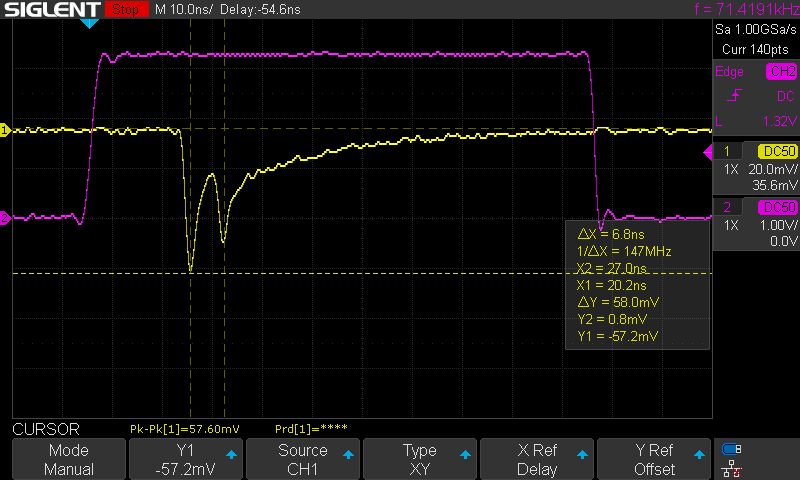
\includegraphics[width=0.49\textwidth]{Grafiken/4-1/Afterpuls}
  \caption{Aufnahme eines Afterpulses}
  \label{AfterpulseGrafik}
\end{figure}



\begin{figure}[h!]
  \centering
  \begin{subfigure}{0.32\textwidth}
    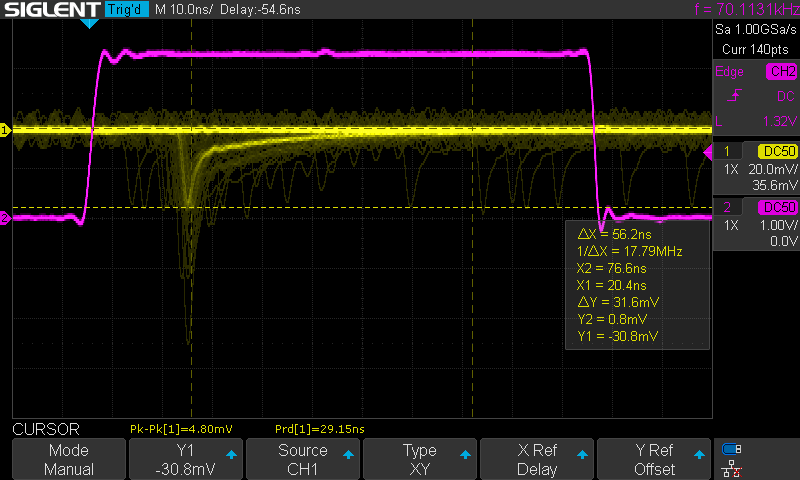
\includegraphics[width=\textwidth]{Grafiken/4-1/4-1-1}
    \caption{Lichtintensität von $2,3$ \& $n_{pe} = 1$}
  \end{subfigure}
  \hfill
  \begin{subfigure}{0.32\textwidth}
    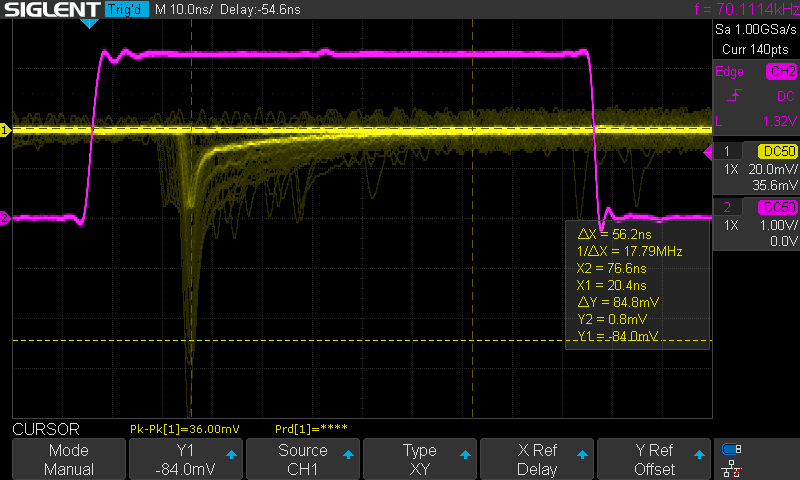
\includegraphics[width=\textwidth]{Grafiken/4-1/4-1-3}
    \caption{Lichtintensität von $2,75$ \& $n_{pe} = 3$}
  \end{subfigure}
  \hfill
  \begin{subfigure}{0.32\textwidth}
    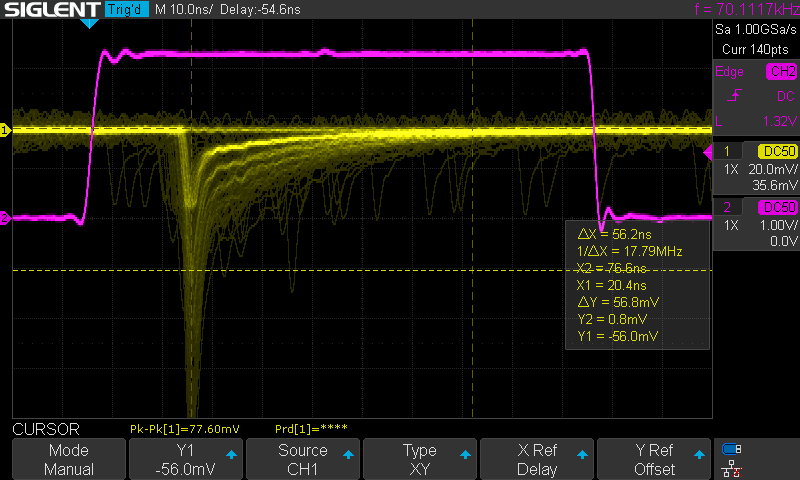
\includegraphics[width=\textwidth]{Grafiken/4-1/4-1-2}
    \caption{Lichtintensität von $3,2$ \& $n_{pe} = 2$}
  \end{subfigure}
  \caption{Oszilloskop-Screenshots bei verschiedenen LED-Intensitäten zum Abmessen der Spannungen für $n_{pe}=[1,2,3]$. Auf dem Oszilloskop sind die entsprechenden einzelnen Linien erkennbar und abhängig von der LED-Intensität auch unterscheidbar.}
  \label{PulseOsziKombi}
\end{figure}


\subsubsection{Anstiegs- und Zerfallszeit}
Um genauere Werte zu erhalten, wurden bei Einzelaufnahmen von verschiedenen Anzahlen $n_{pe}$ von Photon mit der Cursors-Funktion und durch Ablesen die Stärke der Pulse sowie deren Anstiegs- und Zerfallszeit ausgemessen.
Die Anstiegs- und Zerfallszeiten der Pulse variieren je nach gemessener Ereignisse n.
Die Anstiegszeit war sehr kurz und lag im Bereich von wenigen Nanosekunden.
Die Zerfallszeit war länger und aufgrund des Rauschens ungenauer abzulesen.
Da die Werte nur geschätzte werden sollten, ergeben sich aus Abb.~\ref{EinzelpulseOszi} Beispielwerte für die Zeiten:

$t_{Anstieg, n=1} = 2.0ns \pm0.2ns$
\quad $t_{Anstieg, n=2} = 3.0ns \pm0.2ns$  


$t_{Zerfall, n=1} = 25ns \pm2ns$
\quad$t_{Zerfall, n=2} = 75ns \pm2ns$

\begin{figure}[h!]
  \centering
  \begin{subfigure}[t]{0.32\textwidth}
    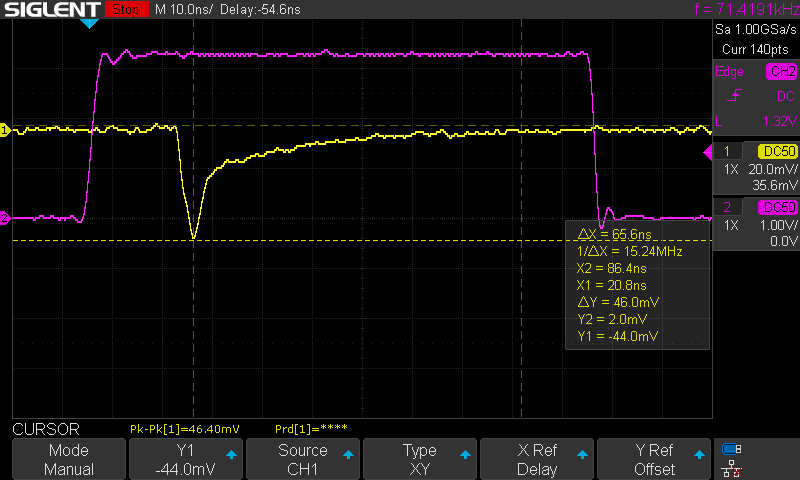
\includegraphics[width=\textwidth]{Grafiken/4-1-2/Zerfall1}
    \caption{Pulse 1}
  \end{subfigure}
  \hfill
  \begin{subfigure}[t]{0.32\textwidth}
    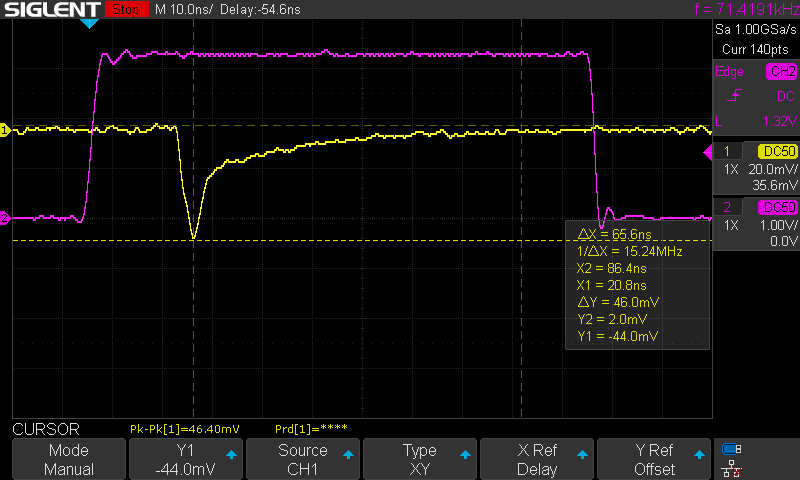
\includegraphics[width=\textwidth]{Grafiken/4-1-2/Zerfall1}
    \caption{Pulse 2}
  \end{subfigure}
  \hfill
  \begin{subfigure}[t]{0.32\textwidth}
    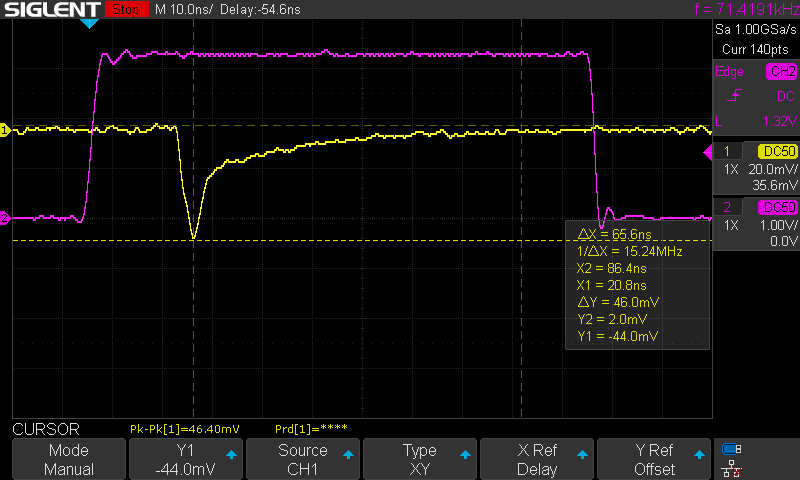
\includegraphics[width=\textwidth]{Grafiken/4-1-2/Zerfall1}
    \caption{Pulse 3}
  \end{subfigure}
  \caption{Auswahl von Aufnahmen einzelner Pulse, auf denen die Anstiegs- und Zerfallszeiten beobachtet werden können. $LI=3,00$ und $U_{Bias}=58V$}
  \label{EinzelpulseOszi}
\end{figure}


\subsubsection{Änderung der Intensität}
Durch das Einstellen einer niedrigen Intensität der LED verschwinden die Peaks vollständig im Rauschen, da der SiPM nicht mehr zwischen den wenigen einzelnen Photonen und den anderen Falschsignalen wie die DCR unterscheiden kann.
Bei höheren Intensitäten steigt die Zahl der detektierten Ereignisse und die Peaks häufen sich und werden größer.


\subsubsection{Spannungsänderung}
Die Bias-Spannung, also die an der Diode angelegte Spannung, ist ein wesentlicher Bestandteil des Experiments.
Um dessen Einfluss besser zu verstehen, haben wir bei gleichbleibender Lichtintensität von $3,00$ verschiedene Spannungen eingestellt und dessen Einfluss auf die Pulse beobachtet.
Bei einer angelegten Spannung von weniger als circa $53V$ waren gar keine Pulse erkennbar bzw. nicht vom Rauschen zu unterscheiden.
Ab $53V$ waren langsam sehr niedrige Pulse zu sehen.
Ab $55V$ waren dann eindeutig die $n_{pe}=1$ Pulse zu sehen und ab $58V$ bereits leicht die $n_{pe}=2$ Pulse.
(Abb.~\ref{SpannungsänderungPuls})

\begin{figure}[h!]
  \centering
  \begin{subfigure}{0.49\textwidth}
    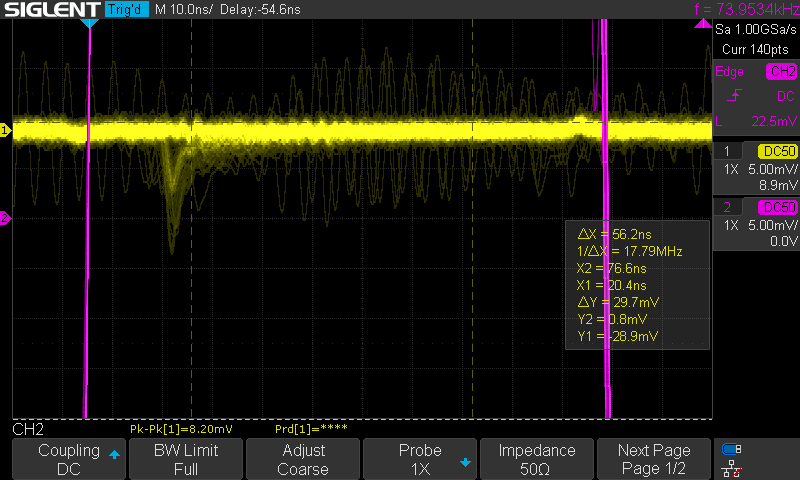
\includegraphics[width=\textwidth]{Grafiken/4-1-4/4-4-53}
    \caption{Pulse bei einer Spannung von $53V$}
  \end{subfigure}
  \hfill
  \begin{subfigure}{0.49\textwidth}
    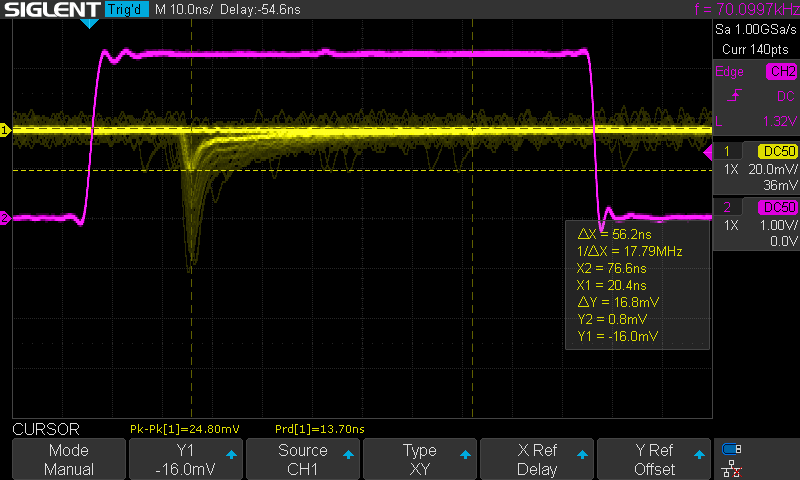
\includegraphics[width=\textwidth]{Grafiken/4-1-4/4-4-55}
    \caption{Pulse bei einer Spannung von $55V$}
  \end{subfigure}
  \hfill
  \begin{subfigure}{0.49\textwidth}
    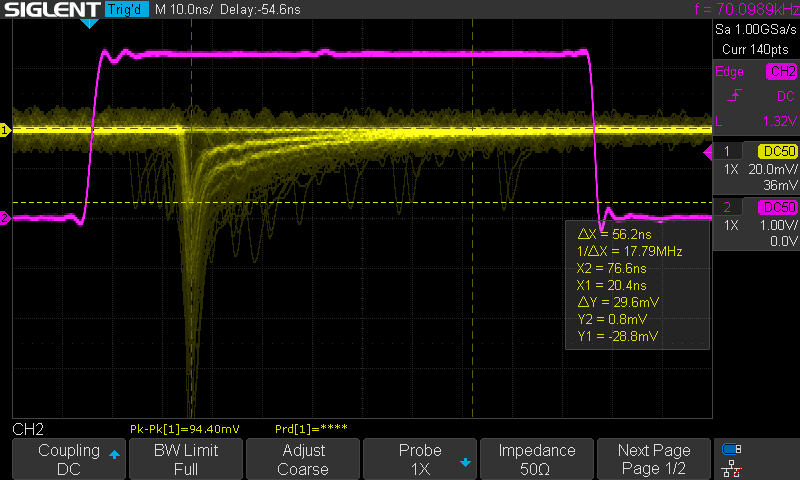
\includegraphics[width=\textwidth]{Grafiken/4-1-4/4-4-58}
    \caption{Pulse bei einer Spannung von $58V$}
  \end{subfigure}
  \hfill
  \begin{subfigure}{0.49\textwidth}
    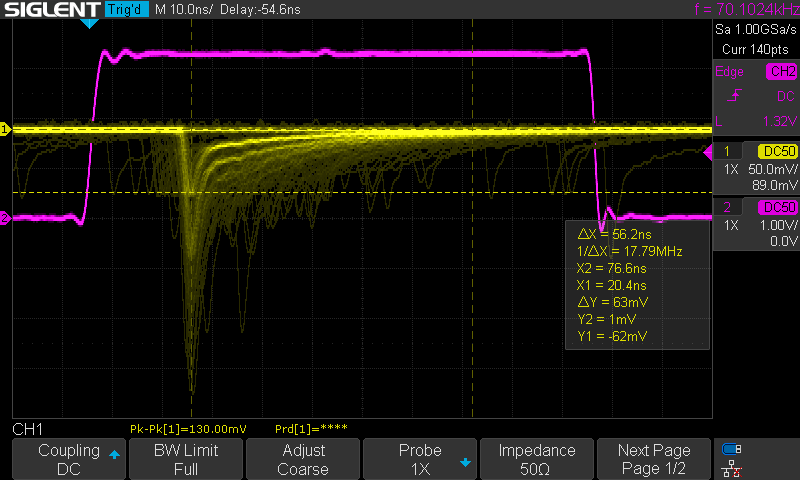
\includegraphics[width=\textwidth]{Grafiken/4-1-4/4-4-65}
    \caption{Pulse bei einer Spannung von $65V$}
  \end{subfigure}
  \caption{Auswahl an Oszilloskopaufnahmen bei einer festen Lichtintensität $3,00$, aber variabler Bias-Spannung}
  \label{SpannungsänderungPuls}
\end{figure}

\subsubsection{Das Gate}
Um nun noch den Einfluss des Gates, des Pre-Gates und der Holdoff Zeit nachvollziehen zu können, haben wir das System so umgebaut, dass der SiPM über seines USB-Anschlusses direkt an den PC angeschlossen war und der Trigger-Out der LED in der Digitizer ging, welcher wiederum an den PC angeschlossen war. Auf dem Computer lief eine LabView Software zum Auswerten der Signale. Dieses Setup wird auch im weiteren Verlauf des Experiments benutzt. \\
Die Gate-Zeit bestimmt, wie groß das Zeitintervall ist, über das integriert wird.
Wenn die Gate-Zeit zu weit erhöht wird, verschwimmen die Peaks.
Bei einer zu geringeren Gate-Zeit verschwinden die Peaks komplett, da die Integrationszeit zu kurz wird, wodurch sich die Integrationsfläche der $0$ annähert.

\begin{figure}[h!]
  \centering
  \begin{subfigure}{0.49\textwidth}
    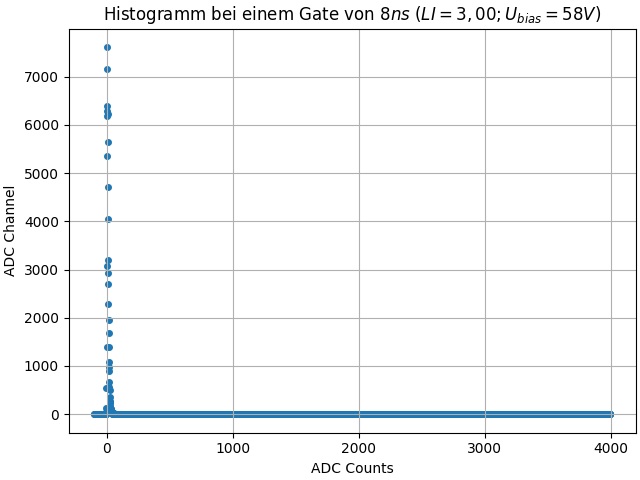
\includegraphics[width=\textwidth]{Grafiken/gate_8}
    \caption{Gate-Zeit von $\tau_{gate} = 8 ns$}
  \end{subfigure}
  \begin{subfigure}{0.49\textwidth}
    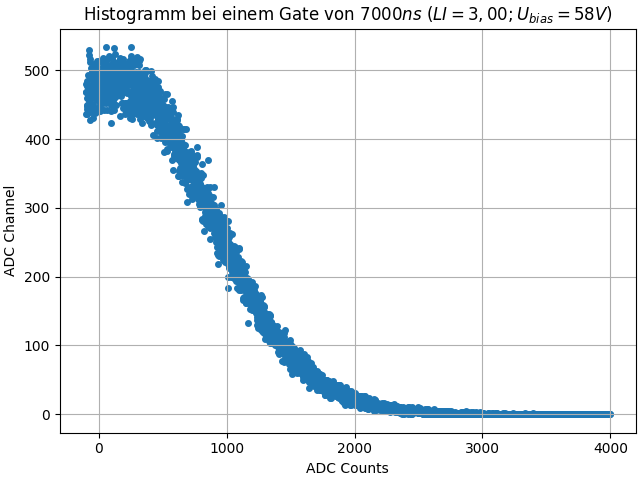
\includegraphics[width=\textwidth]{Grafiken/gate_7000}
    \caption{Gate-Zeit von $\tau_{gate} = 7000 ns$}
  \end{subfigure}
  \caption{Darstellung des Einflusses der Gate-Zeit bei extrem kleinen und großen Wert.}
  \label{GateSpeilen}
\end{figure}

Die Pre-Gate-Zeit bestimmt, wie lange die Software nach Erhalt des Triggersignals der LED wartet, bis angefangen wird, das Sensorsignal zu integrieren.
Die Holdoff-Zeit bestimmt, wie lange nach Abschluss des Integrierens die Software wartet, bevor sie wieder auf den Trigger reagiert.
In diesem Zeitraum passiert nichts.
Die Pre-Gate- und Holdoff-Einstellung sind wichtig, um den Einfluss des Afterpulsings und der DCR auf das Messergebnis zu verringern. Da diese nicht im Takt mit dem Trigger auftreten, wird deren Einfluss auf das Integral auf diese Weise auf einen kleinen Anteil reduziert.
Dies sorgt dafür, dass die Minima im Histogramm ansteigen, dafür verfälschen Sie aber nicht mehr die Peaks des Histogramms.

\subsection{Aufnahme von Dunkel-Spektren}
\subsubsection{Wahrscheinlichkeitsverteilung der DCR}
Die Verteilung der erwarteten Zahl an Photonen, die innerhalb eines gewissen Zeitintervalls detektiert werden, ist Poissonverteilt.
Das liegt daran, dass eine Detektion von mehr Ereignissen gleichzeitig, mit wachsender Anzahl an gleichzeitig gemessenen Ereignissen immer unwahrscheinlicher wird.
Es ist also sehr viel wahrscheinlicher, eine niedrige Anzahl an Ereignissen zu detektieren, als eine hohe.
Das ist charakteristisch für eine Poisson-Verteilung.

\subsubsection{Dunkelspektren für verschiedenen Spannungen}
In Abbildung~\ref{Dunkelspektren} dargestellt, wurden die Dunkelspektren bei einer angelegten Spannung von $57V$, $60V$ und $63V$ aufgenommen.


\begin{figure}[h!]
  \centering
  \begin{subfigure}{0.32\textwidth}
    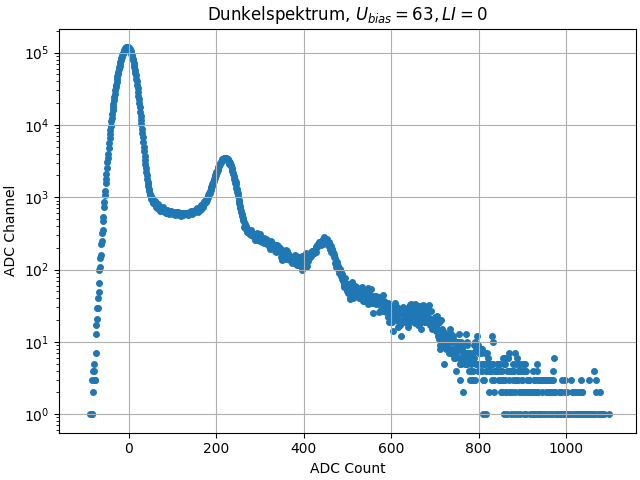
\includegraphics[width=\textwidth]{Grafiken/dunkel_57}
    \caption{$U_{Bias} = 57V$}
  \end{subfigure}
  \hfill
  \begin{subfigure}{0.32\textwidth}
    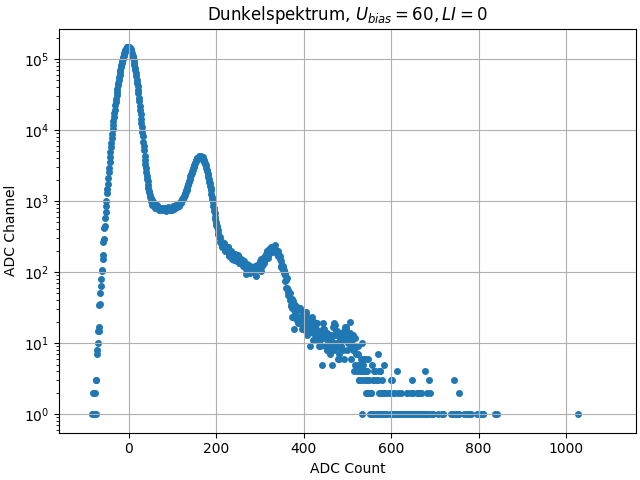
\includegraphics[width=\textwidth]{Grafiken/dunkel_60}
    \caption{$U_{Bias} = 60V$}
  \end{subfigure}
  \hfill
  \begin{subfigure}{0.32\textwidth}
    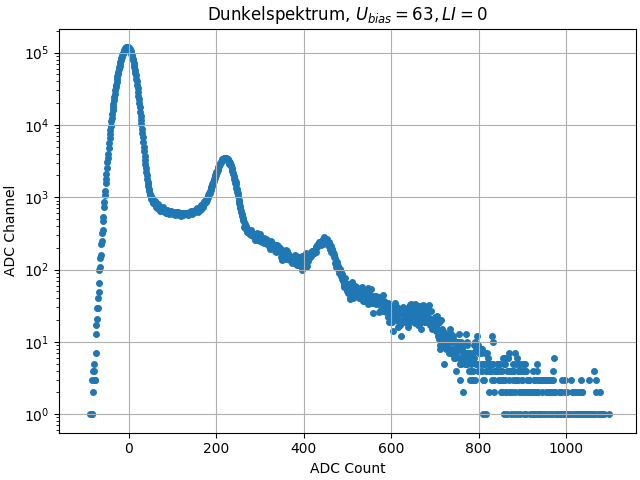
\includegraphics[width=\textwidth]{Grafiken/dunkel_63}
    \caption{$U_{Bias} = 63V$}
  \end{subfigure}
  \caption{Dunkelspektren ($LI=0$) bei verschiedenen angelegten Spannungen.
  y-Achse jeweils logarithmisch skaliert. }
  \label{Dunkelspektren}
\end{figure}

\subsubsection{Methoden zur Bestimmung der DCR}



Die DCR lässt sich aus dem Experiment ermitteln, indem man den Anteil der Ereignisse oberhalb eines halben gefeuerten Pixels bestimmt. Dieser Wert $f_{0.5}$ ist das Verhältnis aus allen Ereignissen über dem halben Gain zu der Summer aller Ereignisse.
Damit folgt für die DCR:
\begin{equation}
    DCR = \frac{f_{0.5}}{\tau_{Gate}}
\end{equation}

Mit den bestimmten Werten für $f_{0.5}$ ergibt sich Tabelle~\ref{DCRBestimmung1}:

\begin{table}[h]
  \begin{center}
    \begin{tabular}{|c|c|c|}
      \hline
      Betriebsspannung [V] & $f_{0.5}$ & DCR [Hz] \\
      \hline
      57 & 0.0355 $\pm 0.0012$ & (3.42 $\pm$ 0.12)$\cdot 10^{5}$ \\
      60 & 0.0461 $\pm 0.0012$ & (4.44 $\pm$ 0.12)$\cdot 10^{5}$ \\
      63 & 0.0538 $\pm 0.0012$ & (5.17 $\pm$ 0.13)$\cdot 10^{5}$ \\
      \hline
    \end{tabular}
    \caption{DCR bestimmt aus $f_{0.5}$ für verschiedene Betriebsspannungen}
    \label{DCRBestimmung1}
  \end{center}
\end{table}


Die DCR lässt sich ebenfalls durch die Annahme einer zugrundeliegenden Poisson-Verteilung bestimmen.
Wenn N die Anzahl der detektierten Dunkel-Ereignisse in der Zeitspanne $\Delta t$ ist, folgt daraus der Erwartungswert der Poisson-Verteilung mit:
\begin{equation}
\lambda = DCR \cdot \Delta t
\end{equation}

Da die Zeitspanne unsere Integrationszeit $\tau_{Gate}$ ist, lässt sich die DCR also bestimmen durch:
\begin{equation}
DCR = \frac{\lambda}{\tau_{Gate}}
\end{equation}
Durch die Annahme einer Poisson-Verteilung gilt:
\begin{equation}
P_{\lambda}(k)=\frac{\lambda^{k}}{k!}e^{-\lambda}\label{PO}
\end{equation}
Mit: $\lambda$: Mittelwert, k: Anzahl Photonen.
Für die DCR, also ohne detektierte Photonen (k = 0) gilt:
\begin{equation}
P_{\lambda}(0)=e^{-\lambda}=\frac{f_{0}}{f_{ges}}
\end{equation}
Mit: $f_{0}$: Anzahl Ereignisse im Pedestal, $f_{ges}$: Anzahl aller Ereignisse.
Der Mittelwert der Poisson-Verteilung, und damit auch die Varianz, lässt sich somit bestimmen durch:
\begin{equation}
\lambda = -ln\frac{f_{0}}{f_{ges}}
\label{PoissonMeanEQ}
\end{equation}
Zusammengesetzt erhalten wir also für die DCR:
\begin{equation}
    DCR = \frac{-ln\frac{f_{0}}{f_{ges}}}{\tau_{Gate}}
\end{equation}
Die so bestimmte DCR liefert folgende Ergebnisse in Tabelle~\ref{DCRBestimmung2}.

\begin{table}[h]
  \begin{center}
    \begin{tabular}{|c|c|}
      \hline
      Betriebsspannung [V] & DCR [Hz] \\
      \hline
      57 & (3.47 $\pm$ 0.06)$\cdot 10^{5}$ \\
      60 & (4.51 $\pm$ 0.07)$\cdot 10^{5}$ \\
      63 & (5.29 $\pm$ 0.08)$\cdot 10^{5}$ \\
      \hline
    \end{tabular}
    \caption{DCR aus Poisson-Annahme für verschiedene Betriebsspannungen}
    \label{DCRBestimmung2}
  \end{center}
\end{table}


Beim Vergleichen der beiden Methoden fällt auf, dass die Ergebnisse der idealen angenommenen Poisson-Verteilung leicht von den anderen Ergebnissen abweichen. Diese Abweichung ist allerdings klein genug, um die angenommene Poisson-Verteilung zu untermauern.

\subsubsection{Crosstalk Wahrscheinlichkeit}
Die Crosstalk Wahrscheinlichkeit können wir über die Correlated Noise [Glg~\ref{CN}] abschätzen.
Wir betrachten hierfür lediglich den prompten Crosstalk, somit ist die Crosstalk Wahrscheinlichkeit durch die Correlated Noise gegeben und wir erhalten die Werte in Tabelle \ref{CorrelatedNoide}

\begin{table}[h]
  \begin{center}
    \begin{tabular}{|c|c|}
      \hline
      Betriebsspannung [V] & CN \\
      \hline
      57 & 0.042 $\pm$ 0.034 \\
      60 & 0.078 $\pm$ 0.026 \\
      63 & 0.105 $\pm$ 0.022 \\
      \hline
    \end{tabular}
    \caption{Correlated Noise für verschiedene Betriebsspannungen}
    \label{CorrelatedNoide}
  \end{center}
\end{table}

\subsection{Aufnahme von LED-Spektren}

\subsubsection{Aufnahme}
Es werden für verschiedenen Betriebsspannungen die LED-Spektren bei einer Intensität von $3,00$ aufgenommen.


\subsubsection{Bestimmung des Gain}
Um den Gain zu bestimmen, wurden - wie in Abb.~\ref{GainBestimmung} zu sehen - für jedes LED-Spektrum in den 0. und 1. Peak eine Gauß-Distribution gefittet. So konnte die Differenz der Faktoren $\mu_{0}$ und $\mu_{1}$, welcher gleich der Gain ist, jeweils bestimmt werden (Glg.~\ref{GainFormel} \& \ref{GainFormelFehler}). Daraus folgten die Werte in Tabelle \ref{GainBestimmtungTabelleEinzeln}

\begin{equation}
    G_i = \mu_{i,1} -  \mu__{i,0}
    \label{GainFormel}
\end{equation}


\begin{equation}
    \Delta G_i = \sqrt{\mu_{i,1}^2 +  \mu_{i,0}^2}
    \label{GainFormelFehler}
\end{equation}

    

\begin{figure}[h!]
  \centering
  \begin{subfigure}{0.32\textwidth}
    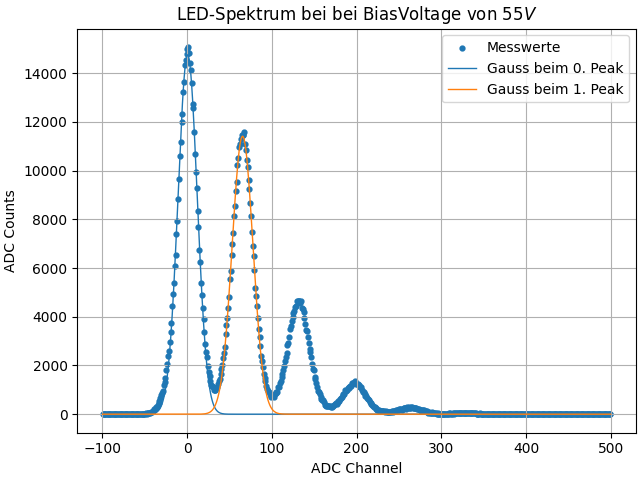
\includegraphics[width=\textwidth]{Grafiken/gaussfit_55}
    \caption{$U_{Bias}=55V$}
  \end{subfigure}
  \hfill
  \begin{subfigure}{0.32\textwidth}
    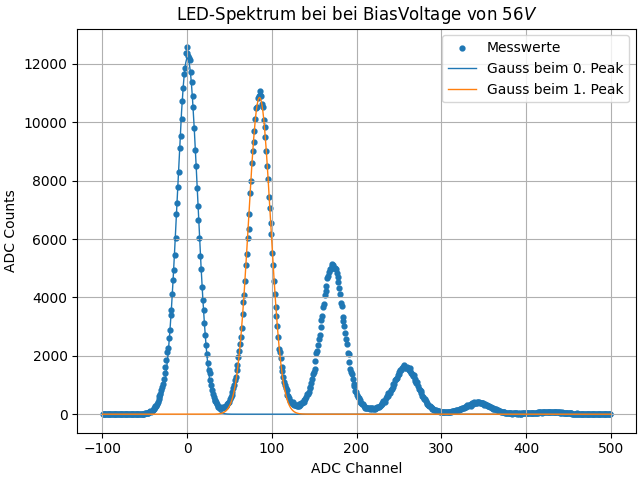
\includegraphics[width=\textwidth]{Grafiken/gaussfit_56}
    \caption{$U_{Bias}=56V$}
  \end{subfigure}
  \hfill
  \begin{subfigure}{0.32\textwidth}
    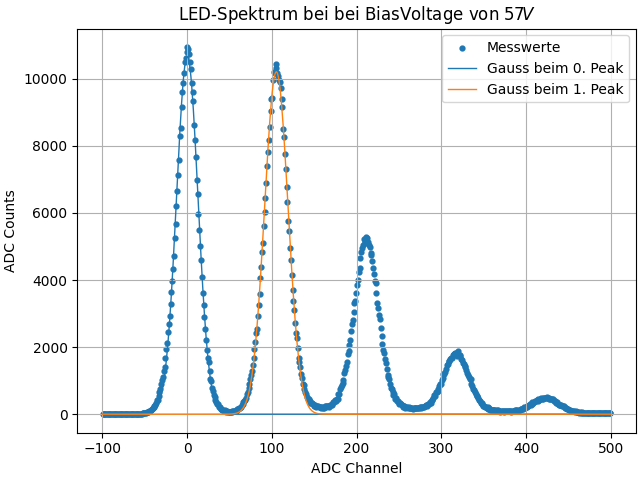
\includegraphics[width=\textwidth]{Grafiken/gaussfit_57}
    \caption{$U_{Bias}=57V$}
  \end{subfigure}
  \hfill
  \begin{subfigure}{0.32\textwidth}
    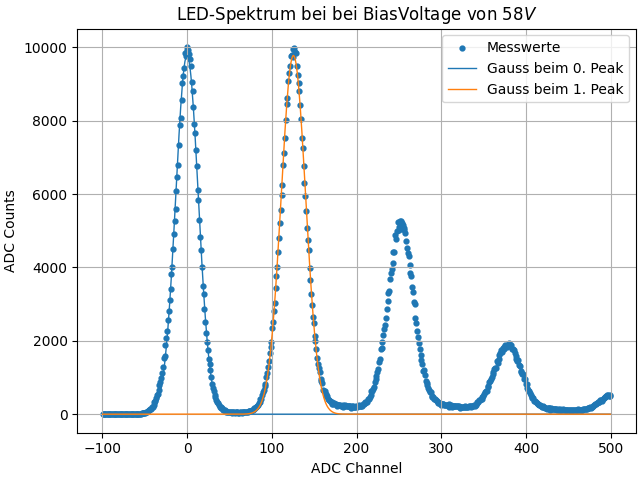
\includegraphics[width=\textwidth]{Grafiken/gaussfit_58}
    \caption{$U_{Bias}=58V$}
  \end{subfigure}
  \hfill
  \begin{subfigure}{0.32\textwidth}
    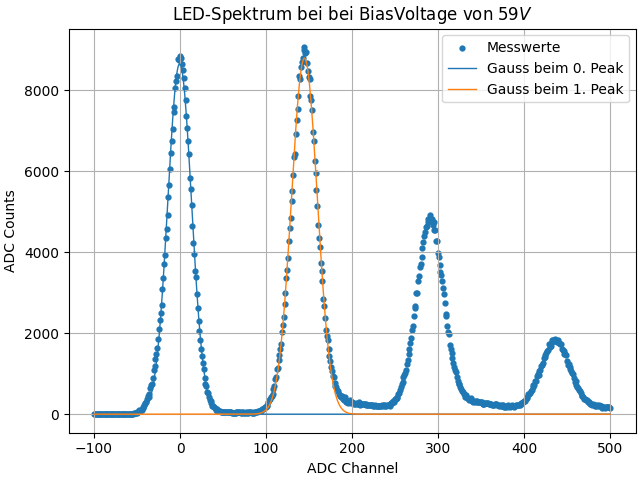
\includegraphics[width=\textwidth]{Grafiken/gaussfit_59}
    \caption{$U_{Bias}=59V$}
  \end{subfigure}
  \hfill
  \begin{subfigure}{0.32\textwidth}
    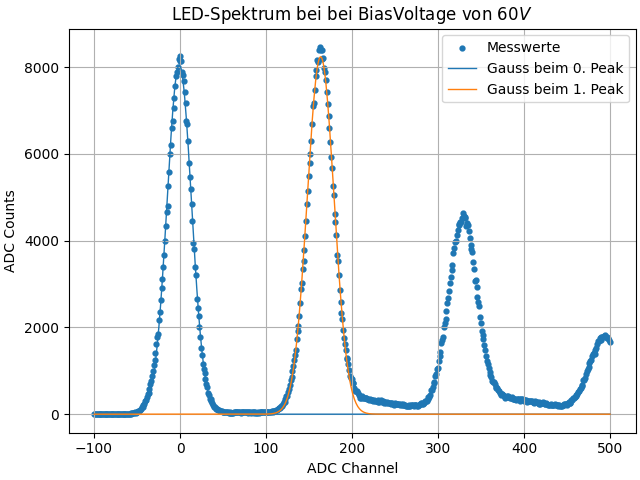
\includegraphics[width=\textwidth]{Grafiken/gaussfit_60}
    \caption{$U_{Bias}=60V$}
  \end{subfigure}
  \hfill
  \begin{subfigure}{0.32\textwidth}
    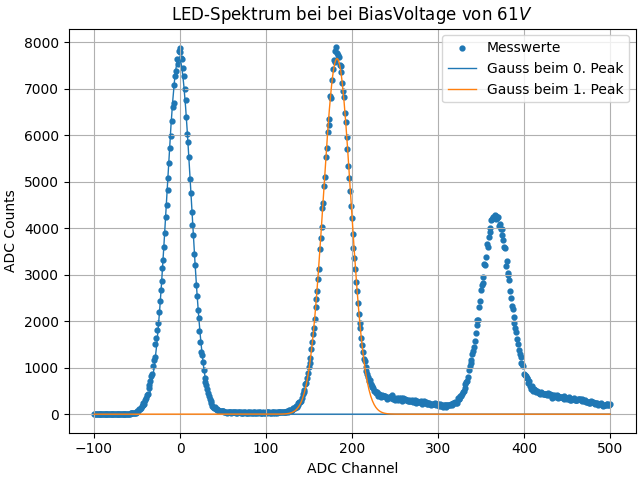
\includegraphics[width=\textwidth]{Grafiken/gaussfit_61}
    \caption{$U_{Bias}=61V$}
  \end{subfigure}
  \begin{subfigure}{0.32\textwidth}
    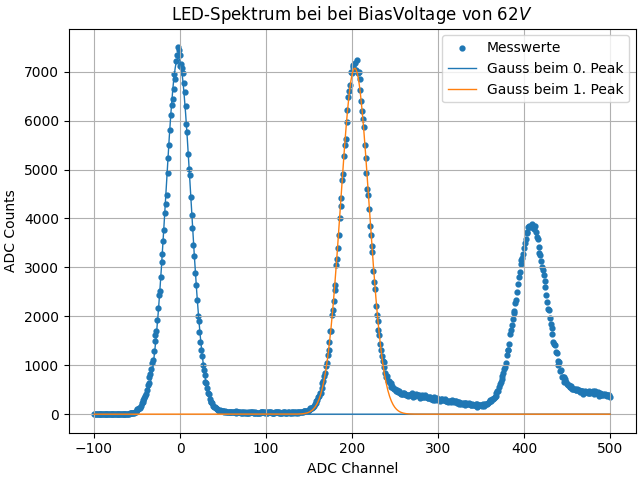
\includegraphics[width=\textwidth]{Grafiken/gaussfit_62}
    \caption{$U_{Bias}=62V$}
  \end{subfigure}
  \hfill
  \caption{Fits der Gauß-Funktionen im 0. und 1. Peak der Histogramme bei verschiedenen $U_{Bias}$ und fester Lichtintensität von $3,00$.}
  \label{GainBestimmung}
\end{figure}



\begin{table}[h]
  \begin{center}
    \begin{tabular}{|c|c|c|c|c|c|c|}
      \hline
      U [V] & $\mu_{0}$ & $\sigma_{0}$ & $\mu_{1}$ &  $\sigma_{1}$ & Gain G [$V^{-1}$] & $\sigma_{G}$ [$V^{-1}$]\\
      \hline
      55 & 1 $\pm$ 4 & 12 $\pm$ 4 & 65 $\pm$ 4 & 13 $\pm$ 4 & 65 & 5 \\
      56 & 0 $\pm$ 4 & 12 $\pm$ 4 & 86 $\pm$ 4 & 13 $\pm$ 4 & 85 & 5 \\
      57 & 0 $\pm$ 4 & 13 $\pm$ 4 & 105 $\pm$ 4 & 14 $\pm$ 4 & 105 & 6 \\
      58 & 0 $\pm$ 4 & 13 $\pm$ 4 & 125 $\pm$ 4 & 14 $\pm$ 4 & 126 & 6 \\
      59 & 0 $\pm$ 4 & 14 $\pm$ 4 & 144 $\pm$ 4 & 15 $\pm$ 4 & 145 & 6 \\
      60 & -1 $\pm$ 4 & 14 $\pm$ 4 & 163 $\pm$ 4 & 16 $\pm$ 4 & 164 & 6 \\
      61 & -1 $\pm$ 4 & 14 $\pm$ 4 & 182 $\pm$ 4 & 16 $\pm$ 4 & 184 & 6 \\
      62 & -2 $\pm$ 4 & 15 $\pm$ 4 & 203 $\pm$ 4 & 17 $\pm$ 4 & 205 & 6 \\
      \hline
    \end{tabular}
    \caption{Gemessene und berechnete Werte zur Bestimmung des Gains.
    \\
    U: Betriebsspannung, $\mu_{0}$: Mittelwert des 0. Peaks, $\sigma_{0}$: Standardabweichung des 0. Peaks, $\mu_{1}$: Mittelwert des 1. Peaks, $\sigma_{1}$: Standardabweichung des 1. Peaks, Gain G: Errechneter Gain, $\sigma_{G}$: Standardabweichung des Gains}
    \label{GainBestimmtungTabelleEinzeln}
  \end{center}
\end{table}

Aus linearer Regression der Gains (Abb.~\ref{GainFit}) ergibt sich der folgende Zusammenhang:
\begin{equation}
    G(U_{Bias}) = (20 \pm1) \frac{(ADC~Channel)}{V} \cdot U_{Bias} - (1030 \pm52)  (ADC Channel)
\end{equation}


\begin{figure}[h!]
  \centering
  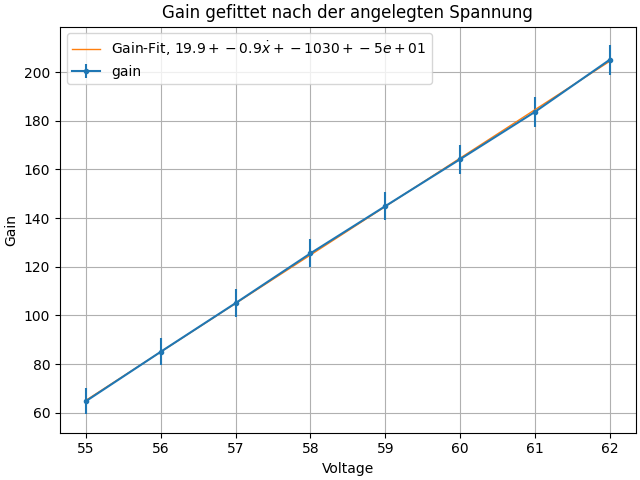
\includegraphics[width=0.49\textwidth]{Grafiken/gain_fit}
  \caption{Fit der Gains mit Fehler}
  \label{GainFit}
\end{figure}





\subsubsection{Mittelwert}

Mit Gleichung~\ref{PoissonMeanEQ} haben wir nun für die, bei verschiedenen angelegten Spannungen aufgenommen, Histogramme den Mittelwert und die Varianz berechnet.
Der Fehler berechnet sich dabei durch

\begin{equation}
\begin{aligned}
\Delta \lambda &= \sqrt{\left( \frac{\partial \lambda}{\partial f_0} \Delta f_0 \right)^2 + \left( \frac{\partial \lambda}{\partial f_{ges}} \Delta f_{ges} \right)^2} \\ &= \sqrt{\left( \left( -(1 / f_{ges} / (f_0 / f_{ges}) ^ 1) \right) \cdot \Delta f_0 \right)^2 + \left( \left( 1 / f_{ges} \right) \cdot \Delta f_{ges} \right)^2}
\end{aligned}
\end{equation}


\begin{table}[h!]
  \begin{center}
    \begin{tabular}{|c|cccccccc|}
      \hline
      $U_{Bias} [V]$ & 55 & 56 & 57 & 58 & 59 & 60 & 61 & 62 \\
      \hline
      $\lambda$& 0.8490 & 0.9796 & 1.0687 & 1.1140 & 1.1456 & 1.1402 & 1.0993 & 1.0840\\
      \hline
      $\sigma_{\lambda}$& 0.0018 & 0.0019 & 0.0020 & 0.0020 & 0.0021 & 0.0021 & 0.0022 & 0.0022\\
      \hline
      
    \end{tabular}
    \caption{Mittelwerte der berechneten Poisson-Verteilung für die angelegten Spannungen bei konstanter Lichtintensität on $LI=3,00$.}
    \label{PoissonMean}
  \end{center}
\end{table}



\subsubsection{Durchbruchsspannung}
Die Durchbruchspannung $V_{bd}$ berechnet sich wie folgt zu:

\begin{align}
V_{bd} &= 51.7287813057 \\
\Delta V_{bd} &= \sqrt{\left( \frac{\partial R}{\partial b} \Delta b \right)^2 + \left( \frac{\partial V_{bd}}{\partial m} \Delta m \right)^2 + \left( \frac{\partial V_{bd}}{\partial y} \Delta y \right)^2} \\
&= \sqrt{\left(-\frac{1}{m}  \cdot \Delta b \right)^2 + \left( -\frac{y - b} { m ^ 2}  \cdot \Delta m \right)^2 + \left( \frac{1}{m} \cdot \Delta y \right)^2} \\&= 3.4726755053  = 3\\
V_{bd} &= \left( 5.2 \pm 0.3 \right) \times 10^{1}
\end{align}

\newpage

\subsection{Modellierung eines LED-Spektrums}
Nun soll ein Modell aufgestellt werden, welches die gemessenen Spektren hinreichend gut beschreibt.
Wie bereits in vorherigen Abschnitten erwähnt, nehmen wir für die Photonanzahl eine Poisson-Verteilung wie [Glg.\ref{PO}] an.

Die auf den Detektor auftreffenden und über die ADC-Channels gemessenen Photonen sind für die verschiedenen Photonzahlen und Channels gaußverteilt und können beschrieben werden durch:
\begin{equation}
    f(x) = \frac{1}{G\cdot \sigma \cdot \sqrt{2\pi}}e^{-0.5\cdot (\frac{x-G\cdot i}{G\cdot \sigma})^{2}}
\end{equation}

Mit: i: Photonenzahl aus Poisson-Verteilung, x: Nummer des ADC-Channels, G: Gain, $\sigma$: Standardabweichung um Peak.
Das $\sigma$ bestimmt sich aus [Glg.\ref{S}].

Um das Modell vollständig aufzustellen, wird für jede Photonenzahl i der erwartete Wert der Poisson-Verteilung mit der aufgestellten Gauß-Verteilung multipliziert und über alle Photonenzahlen summiert, um das gesamte Spektrum abzubilden.
Die Kombination der Gleichungen liefert uns also:
\begin{equation}
    g(\lambda,\sigma,G)(x) = \sum_{i=0}^{\infty}\frac{\lambda^{i}}{i!}e^{-\lambda}\frac{1}{G\cdot \sigma_{i} \cdot \sqrt{2\pi}}e^{-0.5\cdot (\frac{x-G\cdot i}{G\cdot \sigma_{i}})^{2}}\label{M}
\end{equation}

In diesem Modell tauchen mehrere freie Parameter auf, die geschickt abgeschätzt werden müssen um das Modell an die gemessenen Kurven zu den verschiedenen Betriebsspannungen anzupassen.

Die jeweils abgeschätzten Parameter sind $\lambda$, $\sigma$ (bzw. $\sigma_{0}$ und $\sigma_{1}$) und G.

\begin{figure}[h!]
  \centering
  \begin{subfigure}{0.49\textwidth}
    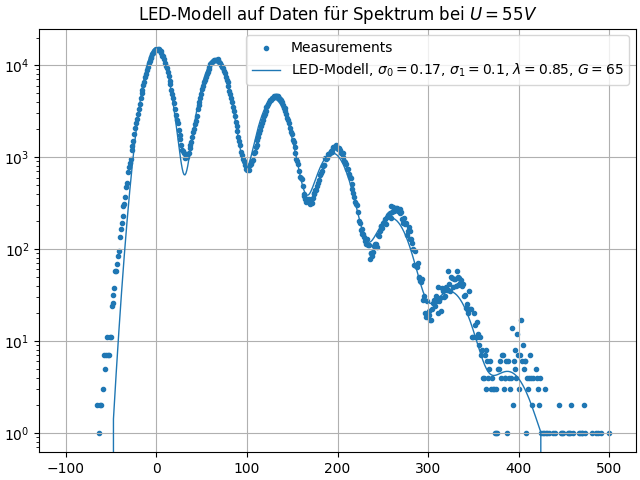
\includegraphics[width=\textwidth]{Grafiken/model 55}
    \caption{$V_{Bias}=55$}
  \end{subfigure}
  \begin{subfigure}{0.49\textwidth}
    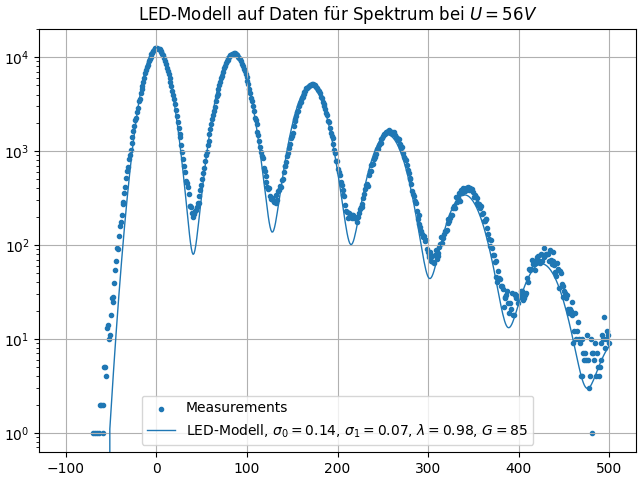
\includegraphics[width=\textwidth]{Grafiken/modell 56}
    \caption{$V_{Bias}=56$}
  \end{subfigure}
  \caption{Darstellung des Modells im direkten Vergleich zu den Messkurven für verschiedenen Betriebsspannungen $V_{Bias}$}
  \label{Modell1}
\end{figure}


\begin{figure}[h!]
  \centering
  \begin{subfigure}{0.49\textwidth}
    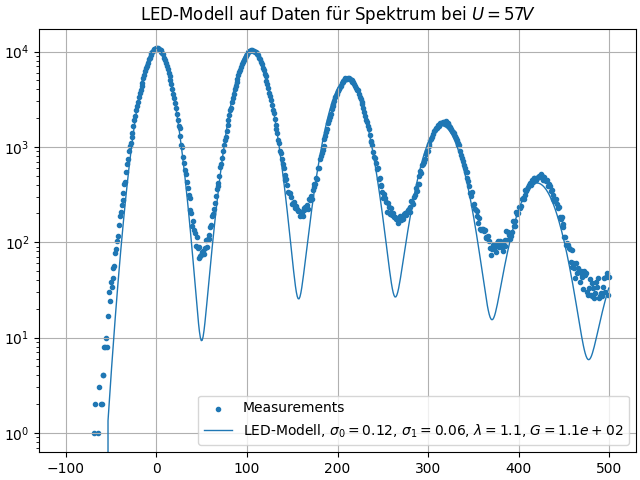
\includegraphics[width=\textwidth]{Grafiken/modell 57}
    \caption{$V_{Bias}=57$}
  \end{subfigure}
  \begin{subfigure}{0.49\textwidth}
    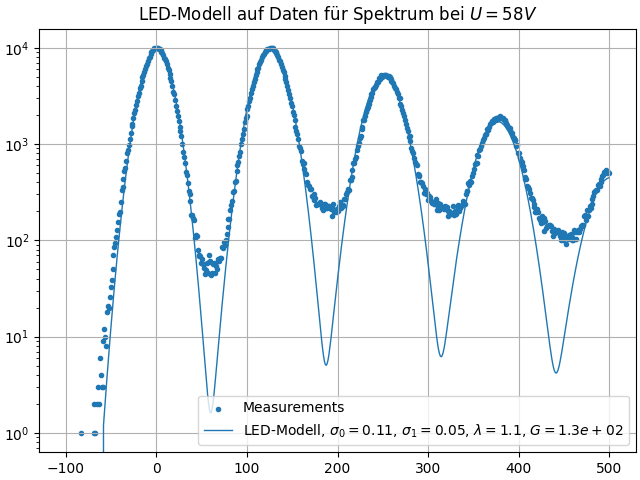
\includegraphics[width=\textwidth]{Grafiken/modell 58}
    \caption{$V_{Bias}=58$}
  \end{subfigure}
  \begin{subfigure}{0.49\textwidth}
    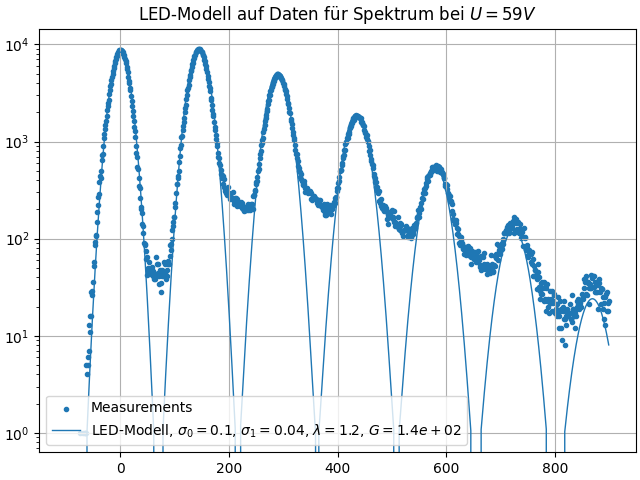
\includegraphics[width=\textwidth]{Grafiken/modell 59}
    \caption{$V_{Bias}=59$}
  \end{subfigure}
  \begin{subfigure}{0.49\textwidth}
    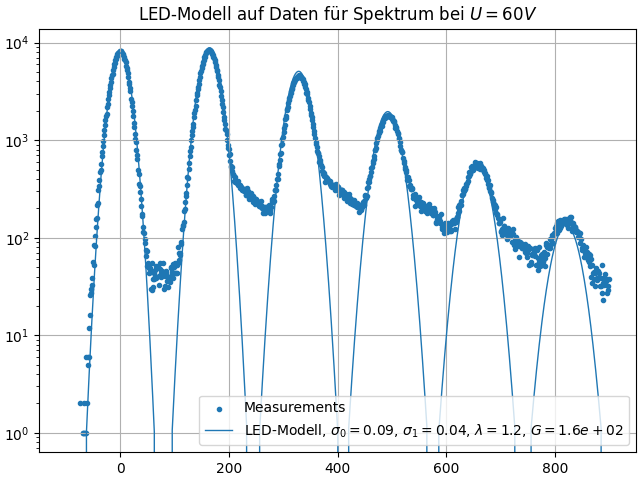
\includegraphics[width=\textwidth]{Grafiken/modell 60}
    \caption{$V_{Bias}=60$}
  \end{subfigure}
  \caption{Weitere Darstellungen des Modells im direkten Vergleich zu den Messkurven für verschiedenen Betriebsspannungen $V_{Bias}$}
  \label{Modell2}
\end{figure}


\begin{figure}[h!]
  \centering
  \begin{subfigure}{0.49\textwidth}
    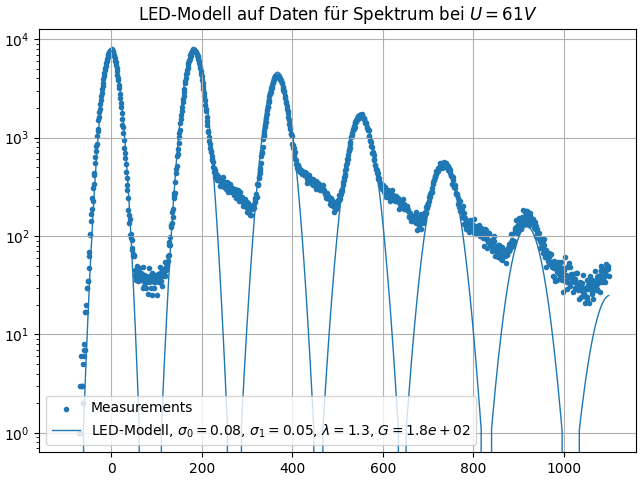
\includegraphics[width=\textwidth]{Grafiken/modell 61}
    \caption{$U_{Bias}=61$}
  \end{subfigure}
  \begin{subfigure}{0.49\textwidth}
    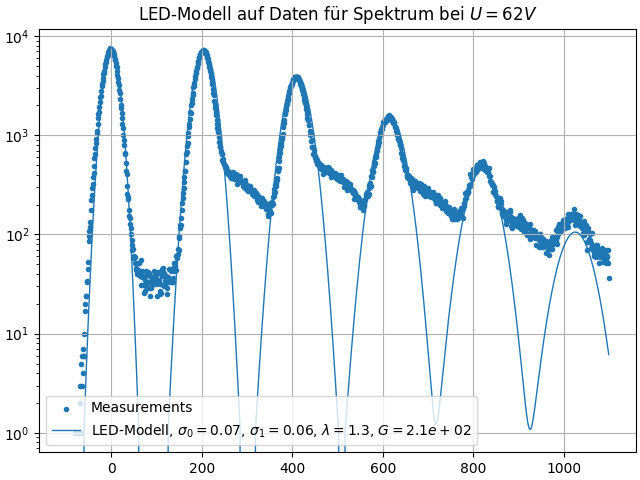
\includegraphics[width=\textwidth]{Grafiken/modell 62}
    \caption{$U_{Bias}=62$}
  \end{subfigure}
  \caption{Weitere Darstellungen des Modells im direkten Vergleich zu den Messkurven für verschiedenen Betriebsspannungen $U_{Bias}$}
  \label{Modell3}
\end{figure}



Um zu überprüfen, wie gut unser aufgestelltes Modell den tatsächlichen Messwerten genügt, wurde ein $X^{2}$-Test durchgeführt.
Im Vorfeld war bereits zu erkennen, dass das Modell die Peaks der Verteilung gut annähern kann, jedoch für mehrzahlige Peaks und höhere Spannung an Genauigkeit verliert.
Der durchgeführte $\chi^{2}$-Test bestätigt diese Beobachtungen und zeigt dennoch, dass eine gute erste Näherung durch das aufgestellte Modell gegeben ist.

Konkret lieferte der $\chi^{2}$-Test die Ergebnisse in Tabelle~\ref{table:Chi2Test}.

\begin{table}[h!]
  \begin{center}
    \begin{tabular}{|c|cccccccc|}
      \hline
      $U_{Bias} [V]$ & 55 & 56 & 57 & 58 & 59 & 60 & 61 & 62 \\
      \hline
      $\chi^{2}$& 244 & 245 & 246 & 253& 245 & 246 & 244 & 244 \\
      \hline
    \end{tabular}
    \caption{Ergebniswerte des $\chi^{2}$-Tests der berechneten LED-Modelle für die, bei verschiedenen angelegten Spannungen gemessenen, Histogramme. $LI=3,00$}
    \label{table:Chi2Test}
  \end{center}
\end{table}


\section{Diskussion}
%Diskussion der physikalischen Ergebnisse.
%Vergleich mit den theoretischen Erwartungen, Fehlerdiskussion.
Die Abweichungen zwischen dem aufgestellten Modell und den realen Messwerten lassen sich gut begründen.
Die abzuschätzenden freien Parameter wurden mehr oder weniger willkürlich gewählt, um sie an unsere Messergebnisse so gut es geht anzupassen und beruhen keinesfalls auf empirischen Daten.
Auch steigt der Gain mit der Spannung zusammen an und sorgt dadurch für größere Lücken zwischen den einzelnen Peaks der modellierten Funktion, in denen der Funktionswert Richtung Null geht. In der Realität gibt es hier allerdings auch weiterhin noch correlated Noise und Dark Counts, die ein tiefes Abfallen des Wertes verhindern.
Weiterhin kommt es natürlich mit erhöhter Spannung auch zu mehr Crosstalk, bzw. correlated Noise im System, was durch unser Modell ebenfalls nicht präzise genug eingefangen wird.
Als letzte Fehlerquelle lässt sich noch das Afterpulsing angeben, durch das die Peaks in der Realität nicht einer perfekten Gauß-Verteilung folgen und so das Modell wieder etwas schlechter machen.


\section{Zusammenfassung}
%Wiederholung/Zusammenfassung der wesentlichen Ergebnisse des Versuchs sowie deren Einordnung. Eventuell Ausblick.
Der Inhalt dieses Kurzversuchs war es sich mit dem Konzept von SiPMs, deren Funktionsweise, Aufbau und Bedingung vertraut zu machen.
Mit diesem Grundlagenwissen sollte anschließend ein Modell ausgearbeitet werden, welches die von einem SiPM aufgenommenen Spektren in guter Näherung beschreiben kann.

\\Zunächst wurden dafür charakteristische Kenngrößen des SiPM variiert und neben der dadurch gewonnenen Intuition wurde auch die Anstiegs- und Zerfallszeit der detektierten Peaks ermittelt.
Die Zeiten liegen für n = 1 bei wenigen Nanosekunden und für n = 2 im zweistelligen Nanosekundenbereich.
Auffällig ist hier, dass die Anstiegs- und Zerfallszeiten zwar von der Anzahl der gleichzeitig detektierten Photonen (n) abhängen, jedoch nicht von der vorher angelegten Betriebsspannung des SiPM.

Die Aufnahme der verschiedenen Spektren für verschiedenen Betriebsspannungen ermöglichte eine Zuordnung der einzelnen Peaks zu dem Auftreten von mehreren gleichzeitigen Photonen im Detektor.
Dadurch ließ sich auch der Verstärkungsfaktor oder Gain G bestimmen und zusätzlich noch die Durchbruchspannung mittels linearer Regression bestimmen $V_{db} = ??? $.
Wenn der SiPM unterhalb dieser Durchbruchspannung betrieben wird, genügt die Energie der Ladungsträger nicht, um einen Lawinenprozess auszulösen.
ie SiPM detektiert dann auch keine Ereignisse.

Als Nächstes wurde über zwei Methoden die DCR ermittelt.
Eine charakteristische Größe des SiPM welche unter anderem die Präzision des Detektors limitiert.
Ebenfalls für Fehler im Detektionsprozess sorgt das Correlated Noise oder die Crosstalk Wahrscheinlichkeit.
Diese wurden weniger exakt, aber auch, ermittelt.

Schlussendlich wurde mit all den vorher bestimmten Daten, Größen und Messwerten ein Modell zur Beschreibung der Spektren eines SiPM aufgestellt.
Dieses Modell basiert auf der Annahme einer Poisson-Verteilung für die Detektion der Photonen kombiniert mit der Näherung der einzelnen Peaks durch eine Gauß-Verteilung [Glg.\ref{M}].
Für verschiedenen Betriebsspannungen funktioniert das Modell in etwa gleich gut.
Entgegen der Erwartung verschlechtert sich das Modell im Vergleich zu den Messwerten, überprüft mit einem $X^{2}$-Test mit steigender Betriebsspannung nicht.
Wie bereits beschrieben müssten sich die Fehlerquellen in der Qualität des Spektrums unseren Erwartungen nach eigentlich mit steigender Betriebsspannung erhöhen.

Eine Verbesserung des Modells wäre möglich, indem man die Poisson-Verteilung zu einer Generalisierten-Poisson-Verteilung ändern würde.
Zusätzlich könnte man noch die Effekte, die die Qualität des Spektrums beeinflussen, wie DCR oder CN, berücksichtigen.

\thispagestyle{empty}

\bibliography{KV4}
\bibliographystyle{unsrt}
\addcontentsline{toc}{chapter}{Bibliography}


[2] V Chmill, E Garutti, R Klanner, M Nitschke, and J Schwandt.
On the characterisation of sipms from pulse-height spectra.
Nuclear Instruments and Methods in Physics Research Section A: Accelerators, Spectrometers, Detectors and Associated Equipment, 854:70–81, 2017

\clearpage
\appendix
\section{Anhang}\label{sec:anhang}
%Hierhin geh\"oren in der Regel Originalmessprotokolle oder weitere Tabellen, die nicht für das Verst\"andnis des Protokolls essentiell sind.

\end{document}
